% PACLock hybrid tokenizer -- architecture schematic for talks.
% Compile: pdflatex tokenizer.tex   (or drop into Overleaf; class standalone)
% Pure ASCII + math mode throughout, standard TikZ libraries only.
\documentclass[tikz,border=8pt]{standalone}
\usepackage{amsmath,amssymb}
\usetikzlibrary{positioning,arrows.meta,calc,fit,backgrounds,decorations.pathreplacing}

\definecolor{rawc}{RGB}{56,108,176}     % raw path
\definecolor{pacc}{RGB}{217,120,44}     % PAC interaction path
\definecolor{gridc}{RGB}{110,110,110}
\definecolor{annot}{RGB}{100,100,100}

\tikzset{
  box/.style={draw=black!55, rounded corners=2pt, fill=black!4,
              align=center, font=\small, inner sep=5pt, minimum height=9mm},
  rawbox/.style={box, draw=rawc, fill=rawc!10},
  pacbox/.style={box, draw=pacc, fill=pacc!10},
  flow/.style={-{Stealth[length=2.2mm]}, thick, black!60},
  rawflow/.style={flow, rawc},
  pacflow/.style={flow, pacc},
  note/.style={font=\scriptsize\itshape, text=annot, align=center},
  lbl/.style={font=\scriptsize, align=center},
}

\begin{document}
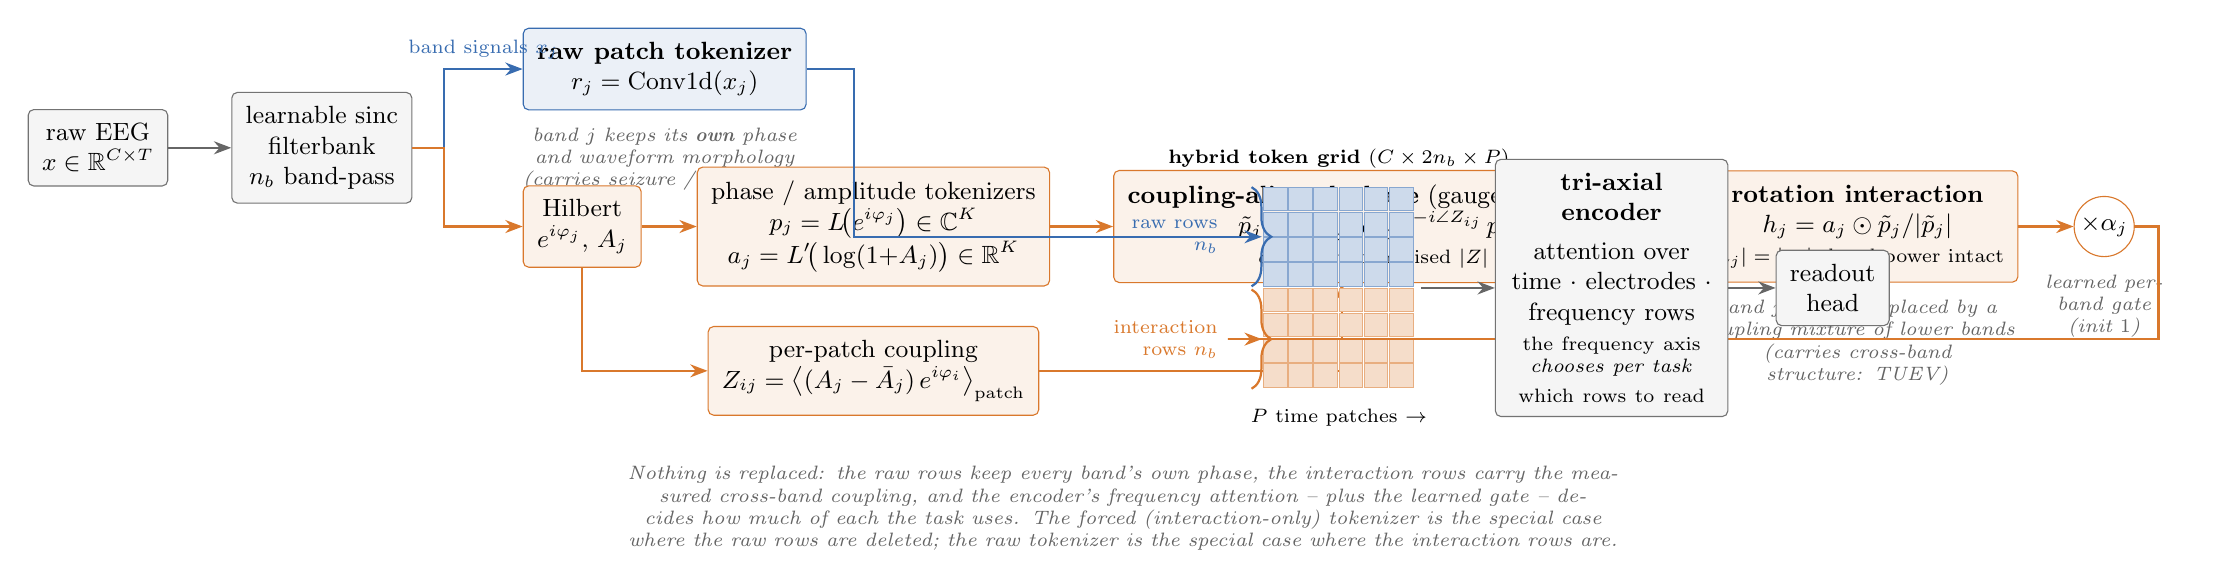
\begin{tikzpicture}[node distance=6mm and 9mm]

% ---------------------------------------------------------------- input
\node[box] (input) {raw EEG\\ $x \in \mathbb{R}^{C\times T}$};

% ---------------------------------------------------------------- filterbank
\node[box, right=8mm of input] (sinc)
  {learnable sinc\\ filterbank\\ $n_b$ band-pass};
\draw[flow] (input) -- (sinc);

% ---------------------------------------------------------------- raw path (top)
\node[rawbox, above right=10mm and 14mm of sinc.east, anchor=west] (rawtok)
  {\textbf{raw patch tokenizer}\\ $r_j=\mathrm{Conv1d}(x_j)$};
\draw[rawflow] (sinc.east) -- ++(4mm,0) |- node[pos=0.75, above, lbl, rawc]
  {band signals $x_j$} (rawtok.west);
\node[note, below=1mm of rawtok, text width=42mm]
  {band $j$ keeps its \textbf{own} phase and waveform morphology\\
   (carries seizure / MI signal)};

% ---------------------------------------------------------------- PAC path (bottom)
\node[pacbox, below right=10mm and 14mm of sinc.east, anchor=west] (hilb)
  {Hilbert\\ $e^{i\varphi_j},\, A_j$};
\draw[pacflow] (sinc.east) -- ++(4mm,0) |- (hilb.west);

\node[pacbox, right=7mm of hilb] (toks)
  {phase / amplitude tokenizers\\
   $p_j = L\!\big(e^{i\varphi_j}\big)\in\mathbb{C}^{K}$\\
   $a_j = L'\!\big(\log(1{+}A_j)\big)\in\mathbb{R}^{K}$};
\draw[pacflow] (hilb) -- (toks);

\node[pacbox, below=5mm of toks] (zbox)
  {per-patch coupling\\
   $Z_{ij}=\big\langle (A_j-\bar A_j)\,e^{i\varphi_i}\big\rangle_{\mathrm{patch}}$};
\draw[pacflow] (hilb.south) |- (zbox.west);

\node[pacbox, right=8mm of toks] (align)
  {\textbf{coupling-aligned phase} (gauge-invariant)\\
   $\tilde p_j=\sum_{i<j}\alpha_{ij}\,e^{-i\angle Z_{ij}}\,p_i$\\
   {\scriptsize $\alpha$ = row-normalised $|Z|$}};
\draw[pacflow] (toks) -- (align);
\draw[pacflow] (zbox.east) -| ($(align.south)+(-4mm,0)$);

\node[pacbox, right=8mm of align] (rot)
  {\textbf{rotation interaction}\\
   $h_j = a_j \odot \tilde p_j / |\tilde p_j|$\\
   {\scriptsize $|h_j|=|a_j|$: band power intact}};
\draw[pacflow] (align) -- (rot);
\node[note, below=1mm of rot, text width=44mm]
  {band $j$'s phase replaced by a coupling mixture of lower bands\\
   (carries cross-band structure: TUEV)};

% ---------------------------------------------------------------- learned gate
\node[circle, draw=pacc, fill=white, inner sep=1.2pt, font=\small,
      right=7mm of rot] (gate) {$\times\alpha_j$};
\draw[pacflow] (rot) -- (gate);
\node[note, below=1mm of gate, text width=24mm]
  {learned per-band gate\\ (init $1$)};

% ---------------------------------------------------------------- hybrid grid
% grid: 8 schematic rows (4 raw + 4 interaction), 6 patch columns
\coordinate (g0) at ($(rawtok.east)+(58mm,-15mm)$);
\foreach \r in {0,1,2,3} {
  \foreach \c in {0,1,2,3,4,5} {
    \fill[rawc!25, draw=rawc!60, line width=0.3pt]
      ($(g0)+(\c*3.2mm, -\r*3.2mm)$) rectangle ++(3.0mm,-3.0mm);
  }
}
\foreach \r in {4,5,6,7} {
  \foreach \c in {0,1,2,3,4,5} {
    \fill[pacc!25, draw=pacc!60, line width=0.3pt]
      ($(g0)+(\c*3.2mm, -\r*3.2mm)$) rectangle ++(3.0mm,-3.0mm);
  }
}
\coordinate (gtop) at ($(g0)+(9.6mm,1.2mm)$);
\node[lbl, anchor=south] at (gtop)
  {\textbf{hybrid token grid} $(C \times 2n_b \times P)$};
% braces
\draw[decorate, decoration={brace, amplitude=2.5mm}, rawc, thick]
  ($(g0)+(-1.5mm,0)$) -- ($(g0)+(-1.5mm,-12.6mm)$)
  node[midway, left=3mm, lbl, rawc, align=right] {raw rows\\ $n_b$};
\draw[decorate, decoration={brace, amplitude=2.5mm}, pacc, thick]
  ($(g0)+(-1.5mm,-13.0mm)$) -- ($(g0)+(-1.5mm,-25.6mm)$)
  node[midway, left=3mm, lbl, pacc, align=right] {interaction\\ rows $n_b$};
\coordinate (gbot) at ($(g0)+(9.6mm,-27.0mm)$);
\node[lbl, anchor=north] at (gbot) {$P$ time patches $\rightarrow$};

% arrows into the grid
\draw[rawflow] (rawtok.east) -- ++(6mm,0) |- ($(g0)+(-4.5mm,-6.3mm)$)
  -- ($(g0)+(-0.2mm,-6.3mm)$);
\draw[pacflow] (gate.east) -- ++(3mm,0) |- ($(g0)+(-4.5mm,-19.3mm)$)
  -- ($(g0)+(-0.2mm,-19.3mm)$);

% ---------------------------------------------------------------- encoder
\coordinate (gmidR) at ($(g0)+(19.4mm,-12.8mm)$);
\node[box, anchor=west, minimum height=26mm, text width=26mm]
  (enc) at ($(gmidR)+(10mm,0)$)
  {\textbf{tri-axial encoder}\\[1mm]
   attention over\\ time $\cdot$ electrodes $\cdot$\\ frequency rows\\[1mm]
   {\scriptsize the frequency axis\\ \emph{chooses per task}\\ which rows to read}};
\draw[flow] ($(g0)+(20.0mm,-12.8mm)$) -- (enc.west);
\node[box, right=6mm of enc, minimum height=9mm] (head) {readout\\ head};
\draw[flow] (enc) -- (head);

% ---------------------------------------------------------------- footnote
\node[note, text width=150mm, anchor=north west]
  at ($(hilb.south west)+(0,-24mm)$)
  {Nothing is replaced: the raw rows keep every band's own phase, the
   interaction rows carry the measured cross-band coupling, and the encoder's
   frequency attention -- plus the learned gate -- decides how much of each the
   task uses. The forced (interaction-only) tokenizer is the special case
   where the raw rows are deleted; the raw tokenizer is the special case where
   the interaction rows are.};

\end{tikzpicture}
\end{document}
